\section{Data generator}

Machine learning models need a fair amount of data examples for training. In supervised learning, each training example consists of input data and target value. In out case input data point is series of pictures captured by telescope and target value is tracklet of object. Not many of these pairs picture series, tracklet are available for training. If we want to train Deep neural network we need to make artificial training data.

\subsection{starGen.r}

The Department of Astronomy and Astrophysics has provided existing solution for this problem. \textbf{StarGen} script is written in language R and is capable of generating single FITS image. It has adjustable parameters:
\begin{itemize}
    \item \textbf{dimX, dimY} - representing size of image
    \item \textbf{starCount} - number of generated stars
    \item \textbf{fwhm} - full width at half maximum (size of star)
    \item \textbf{briMin, briMax} - brightness parameters
    \item \textbf{method} - method used for star generation, gauss, cauchy, line
\end{itemize}

Script is able to generate FITS images with set number of stars. Stars can be seen as point light source or line which simulates telescope movement. 


\begin{figure}[!h]
\centering
\begin{subfigure}{.5\textwidth}
  \centering
  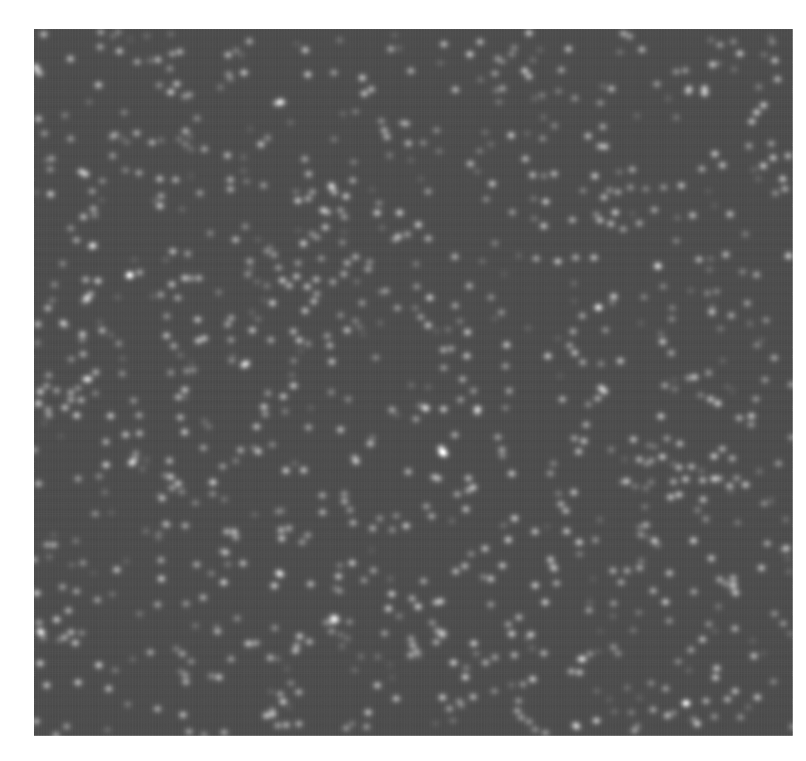
\includegraphics[width=1.0\linewidth]{front_pages/images/original_star_gen.png}
  \caption{Image with 1000 stars and fwhm 10}
  \label{fig:star_gen_orig}
\end{subfigure}%
\begin{subfigure}{.5\textwidth}
  \centering
  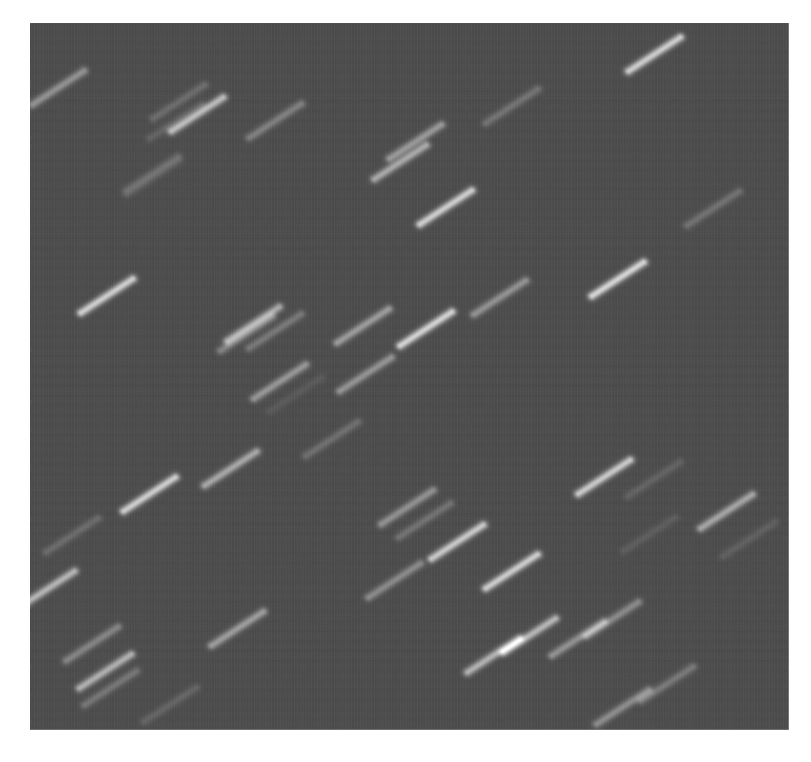
\includegraphics[width=1.0\linewidth]{front_pages/images/original_star_gen_lines.png}
  \caption{Image with lines, 10 fwhm, 50 stars }
  \label{fig:star_gen_orig_lines}
\end{subfigure}
\caption{Images generated by starGen.r}
\label{fig:star_gen}
\end{figure}

\subsection{StarGen.py}

\textit{starGen.r} generates images which cant be directly used as training examples for machine learning models. Whole script was rewritten to Python and modified. 

\begin{itemize}
    \item \textbf{Series of images} \\
    For training data we need series of images not only one image. New generator generates image series of length 8.
    
    \begin{figure}[!h]
    \centering
    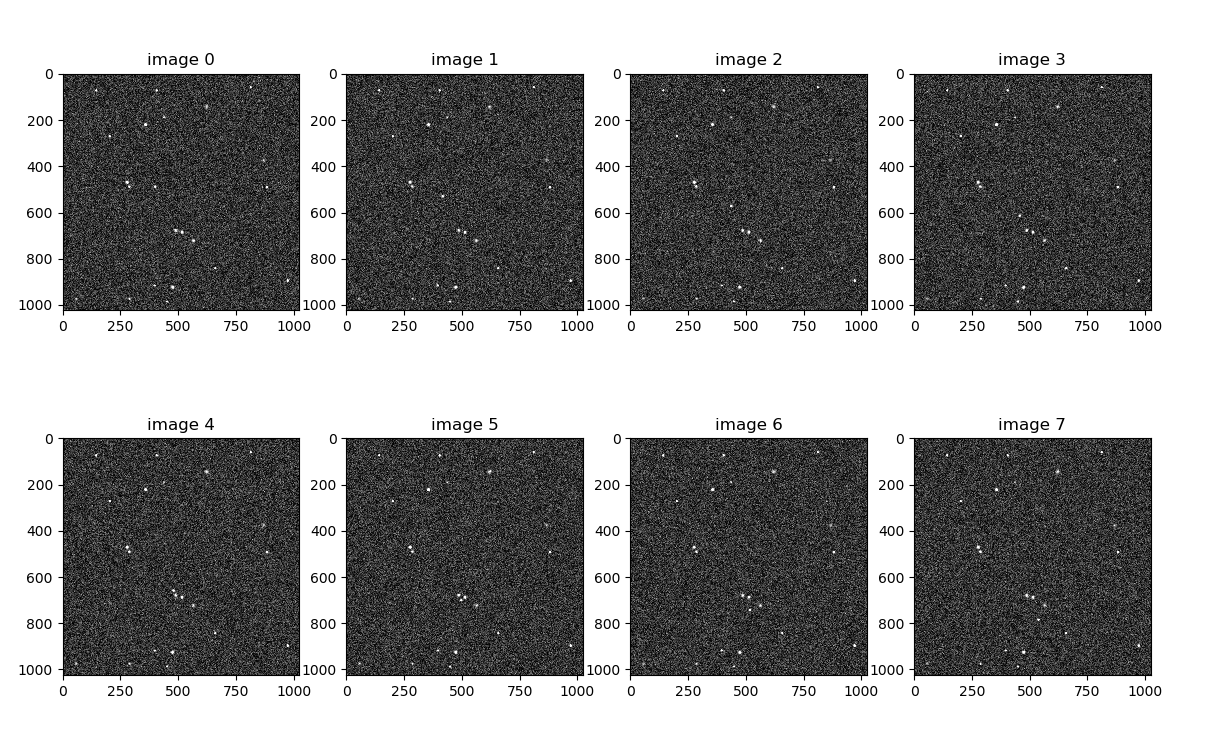
\includegraphics[width=150mm]{chapters/images/data_series.PNG}
    \caption{Series of 8 images created by generator}
    \label{fig:series_data_generator}
    \end{figure}
    
    \item \textbf{Objects}\\
    Original script is not producing tracking object in the picture. We have modified script to produce variable number of objects and their trajectories. Trajectory consists of object positions in each image of the series.
    
    \begin{figure}[!h]
    \centering
    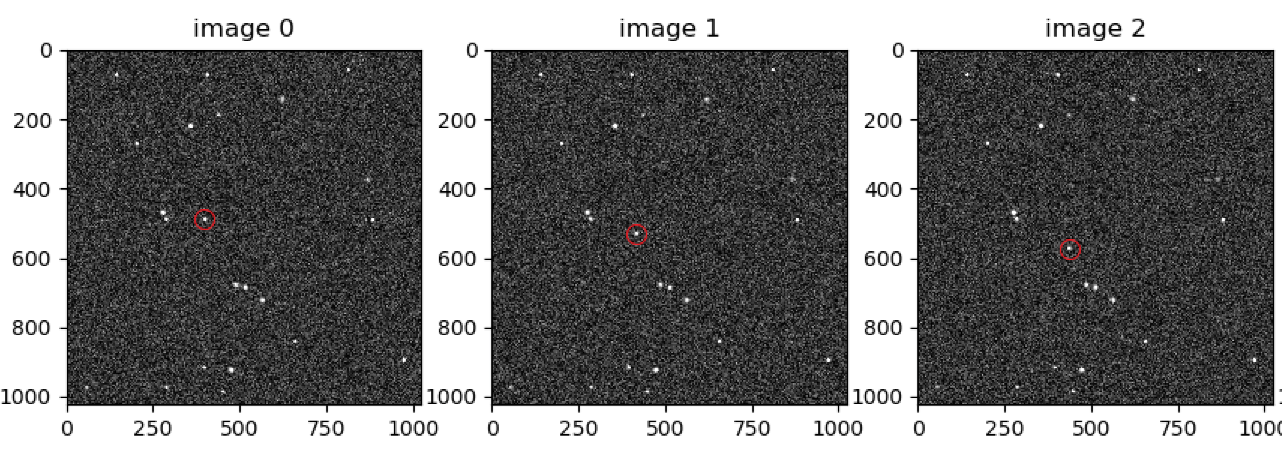
\includegraphics[width=1.0\linewidth]{chapters/images/cast_seria_object_vyznaceny.PNG}
    \caption{Moving object in images}
    \label{fig:object_data_generator}
    \end{figure}
    
    \item \textbf{TSV output file}\\
    Positions of both stars and object in each frame are stored to \textit{.tsv} file with same structure as after \textbf{Segmentation} step in existing system \ref{chap:overview}. This ensures that artificial data will be compatible with real data.
    Files contains one extra Boolean field for marking object position.
    
    
    \begin{figure}[!h]
    \centering
    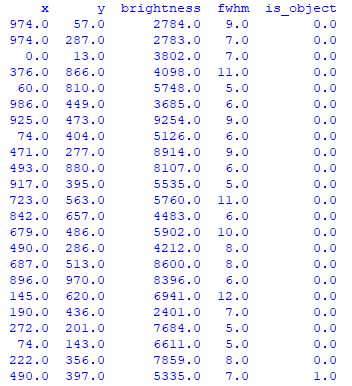
\includegraphics[height=100mm]{chapters/images/tsv_file.PNG}
    \caption{Tsv file representing positions of stars and objects}
    \label{fig:tsv_file_data_generator}
    \end{figure}
    
    \item \textbf{Point objects}\\
    For training purposes and simplicity, script is generating only point light sources.
    
\end{itemize}

Parameters for script are stored in \textit{config.yml} file. We can set: number of series, number of objects and stars in frame, stars and object paramaters. Script produce set number of series consisting of eight FITS images and eight .tsv files.






 


